\documentclass{article}

% \usepackage[latin1]{inputenc}
\usepackage[french]{babel}
\usepackage[T1]{fontenc}

\usepackage{lastpage}
\usepackage{fancyhdr}
\usepackage{graphicx}
\usepackage{pdflscape}

\usepackage[a4paper, margin=2.2cm, footskip=12.3pt]{geometry}

\setcounter{secnumdepth}{0}

\newcommand{\header} {
    \setlength{\headheight}{30pt}\pagestyle{fancy}
    \fancyhead[L]{
\includegraphics[height=20pt]{../logo.pdf}}\fancyhead[C]{}
    \fancyhead[R]{Vitória Cosmo, Aubry Mangold, Eva Ray\\\today}\fancyfoot[C]{}
    \fancyfoot[R]{Page \thepage~sur \pageref{LastPage}}\renewcommand{\footrulewidth}{0.3pt}
}

\title{Gestion d'un service de réparation d'objets\\[1ex]Modélisation conceptuelle}
\author{Vitória Cosmo, Aubry Mangold, Eva Ray}
\date{29 octobre 2023}

\begin{document}
\header


\maketitle

\pagebreak
\begin{landscape}
\begin{figure}[!htb]
        \centering
        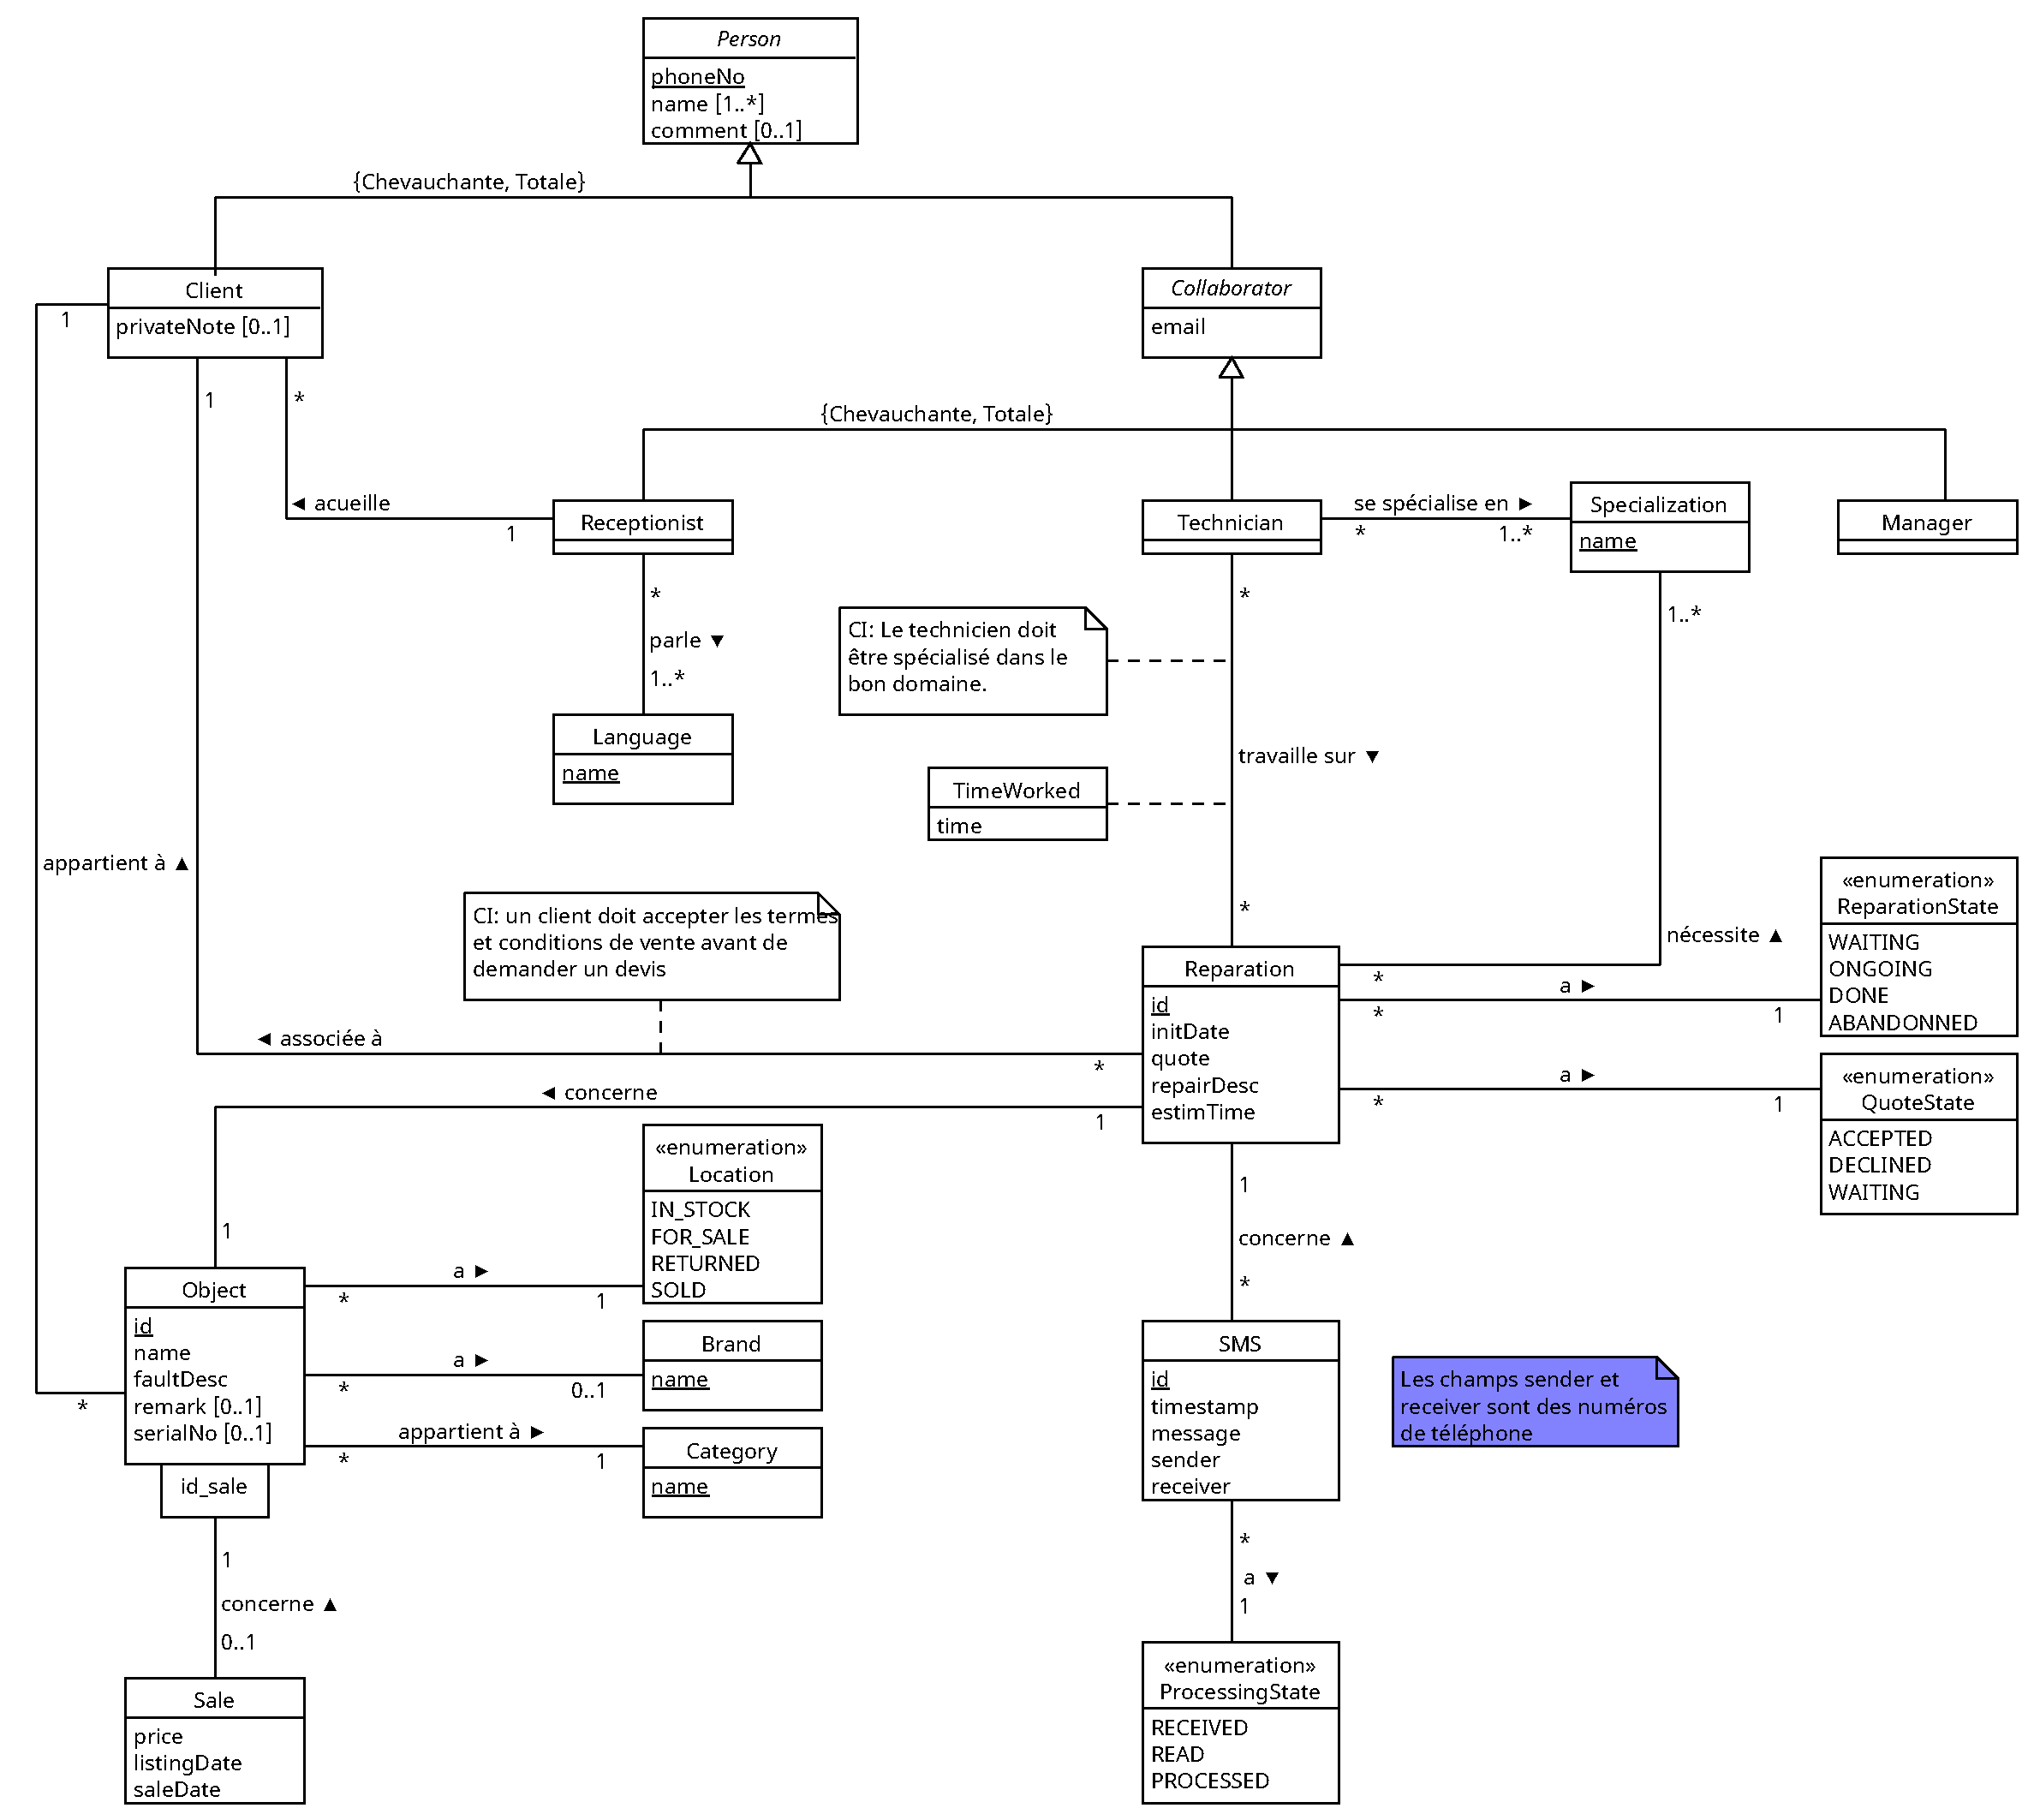
\includegraphics[height=0.93\textheight]{../assets/uml.pdf}
        \caption{Schéma conceptuel de la base de données.}
\end{figure}
\end{landscape}

\pagebreak

\section{Contraintes d'intégrité}

\begin{itemize}
    \item Un client doit accepter les termes et conditions de vente avant de demander un devis.
    \item Le technicien doit être spécialisé dans le bon domaine.
    \item Si \texttt{QuoteState} est \texttt{WAITING}, alors \texttt{ReparationState} est \texttt{WAITING} et \texttt{Location} est \texttt{IN\_STOCK}.
    \item \texttt{Sale} n'existe que si \texttt{QuoteState} est \texttt{DECLINED}.
    \item Si \texttt{Location} est \texttt{FOR\_SALE} ou \texttt{SOLD}, alors \texttt{Quote} doit être \texttt{DECLINED}.
    \item Si \texttt{ReparationState} est \texttt{ONGOING} ou \texttt{DONE}, alors \texttt{QuoteState} est \texttt{ACCEPTED}.
\end{itemize}

\pagebreak
\section{Modifications}

\subsection*{Révision du 16.11.2023}

\begin{itemize}
    \item Renommage de la table \texttt{Client} en \texttt{Customer}.
    \item Suppression de la relation \texttt{accueille} entre les tables \texttt{Client} et \texttt{Receptionist}.
    \item Ajout de la relation \texttt{cree} entre les tables {Receptionist} et {Reparation}
    \item Ajout du membre \texttt{tosAccepted} dans la table \texttt{Client}.
    \item Ajout des contraintes d'intégrité.
\end{itemize}

\end{document}